\subsection{スペクトログラムのパラメータ感度の定量評価}

5.2 節では、課題 5 のスペクトログラムのパラメータ(窓長・窓関数・表示スケール)が
メッセージの判読性に与える影響を定性的に述べた。本節では、追加実験
{\tt exp02\_spectrogram.py} により、この影響を画像コントラスト指標で定量化した
結果を考察する。実験ソースコードと実行出力の全文は付録に無加工で示す。

\subsubsection{実験方法とコントラスト指標の定義}

report\_audio.wav(標本化周波数 $f_s = 44100$ Hz、264600 サンプル、6.00 秒)に
対して、{\tt scipy.signal.spectrogram}\cite{b2-scipy} を用いて以下の 3 系列の
設定でスペクトログラムを計算した。

\begin{itemize}
\item 窓長 {\tt nperseg} $\in \{128, 512, 1024, 4096, 16384\}$
      (ハン窓、オーバーラップは窓長の 75\% に固定)
\item 窓関数 $\in \{$hann, boxcar, blackman$\}$({\tt nperseg} $= 1024$ に固定)
\item 表示スケール $\in \{$dB, 線形$\}$({\tt nperseg} $= 1024$、ハン窓に固定)
\end{itemize}

判読性の定量指標には、実際に紙面に表示される濃淡そのものを対象とするため、
表示画素値を用いた。dB 表示ではパワーの dB 値(式 \ref{eq:db})を、
最大値 $P_{\max}$ からダイナミックレンジ $D = 80$ dB の範囲で
$[0, 1]$ に正規化した値
\begin{equation}\label{eq:b2-norm}
I(m,k) = \min\!\left(1,\ \max\!\left(0,\
\frac{P_{\mathrm{dB}}(m,k) - (P_{\max} - D)}{D}\right)\right)
\end{equation}
を表示画素値と定義する($m$ は時間格子、$k$ は周波数ビン)。これは図の
{\tt pcolormesh} に与える表示範囲({\tt vmin} $= P_{\max} - D$、
{\tt vmax} $= P_{\max}$)と同一の規則であり、図の見た目と指標が対応する。
線形表示では $I(m,k) = S(m,k)/S_{\max}$($S$ はパワー、$S_{\max}$ はその最大値)
とした。

メッセージが目視で確認できる帯域 1--12 kHz の画素集合を $B$ とし、
2 つのコントラスト指標を定義した。第 1 は RMS コントラスト
\begin{equation}\label{eq:b2-rms}
C_{\mathrm{RMS}} = \sqrt{\frac{1}{|B|} \sum_{(m,k) \in B}
\left( I(m,k) - \bar{I} \right)^2}
\end{equation}
($\bar{I}$ は帯域内平均)であり、表示濃淡の広がりを直接測る。第 2 は
外れ値に頑健な 5/95 パーセンタイル版のミケルソンコントラスト
\begin{equation}\label{eq:b2-mic}
C_{\mathrm{M}} = \frac{I_{95} - I_{5}}{I_{95} + I_{5}}
\end{equation}
($I_{95}$、$I_{5}$ は帯域内画素値の 95、5 パーセンタイル)である。
全設定の測定結果を表 \ref{tab:b2-contrast} に示す。表中の $\Delta f = f_s/N$ は
周波数ビン間隔、$\Delta t = H/f_s$($H = N/4$ はホップ幅)は時間格子間隔である。

\begin{table}[htbp]
\centering
\caption{STFT パラメータごとのコントラスト指標(帯域 1--12 kHz。
基準設定 hann、{\tt nperseg} $=1024$、dB は各区分に重複して現れる)}
\label{tab:b2-contrast}
\begin{tabular}{llrrrrrr}
\hline
区分 & 窓関数 & スケール & {\tt nperseg} & $\Delta f$ [Hz] & $\Delta t$ [ms] &
$C_{\mathrm{RMS}}$ & $C_{\mathrm{M}}$ \\
\hline
窓長 & hann & dB & 128 & 344.53 & 0.726 & 0.2995 & 0.9292 \\
窓長 & hann & dB & 512 & 86.13 & 2.902 & 0.2966 & 1.0000 \\
窓長 & hann & dB & 1024 & 43.07 & 5.805 & 0.2719 & 1.0000 \\
窓長 & hann & dB & 4096 & 10.77 & 23.220 & 0.2422 & 1.0000 \\
窓長 & hann & dB & 16384 & 2.69 & 92.880 & 0.1961 & 1.0000 \\
窓関数 & hann & dB & 1024 & 43.07 & 5.805 & 0.2719 & 1.0000 \\
窓関数 & boxcar & dB & 1024 & 43.07 & 5.805 & 0.1617 & 0.4101 \\
窓関数 & blackman & dB & 1024 & 43.07 & 5.805 & 0.3063 & 1.0000 \\
スケール & hann & dB & 1024 & 43.07 & 5.805 & 0.2719 & 1.0000 \\
スケール & hann & 線形 & 1024 & 43.07 & 5.805 & 0.2230 & 1.0000 \\
\hline
\end{tabular}
\end{table}

なお、図 \ref{fig:b2-nperseg} から分かるように、本音声のメッセージは
「明るい背景(広帯域雑音)から文字形状にエネルギーを欠落させた」
ノッチ型の埋め込みであり、文字は白地に黒く現れる。以下の考察は
この埋め込み形態を前提とする。

\subsubsection{窓長の感度と不確定性関係}

窓長を変えた 5 設定のスペクトログラムを図 \ref{fig:b2-nperseg} に、
コントラスト指標の推移を図 \ref{fig:b2-contrast} に示す。
$C_{\mathrm{RMS}}$ は {\tt nperseg} $= 128$ の 0.2995 から
16384 の 0.1961 まで単調に減少し、最小設定と最大設定の間で約 35\% 低下した。
図 \ref{fig:b2-nperseg} の目視でも、4096 で文字の時間方向のにじみが現れ、
16384 では文字がほぼ塗りつぶされて判読困難となっており、指標の低下と一致する。

\begin{figure}[p]
\centering
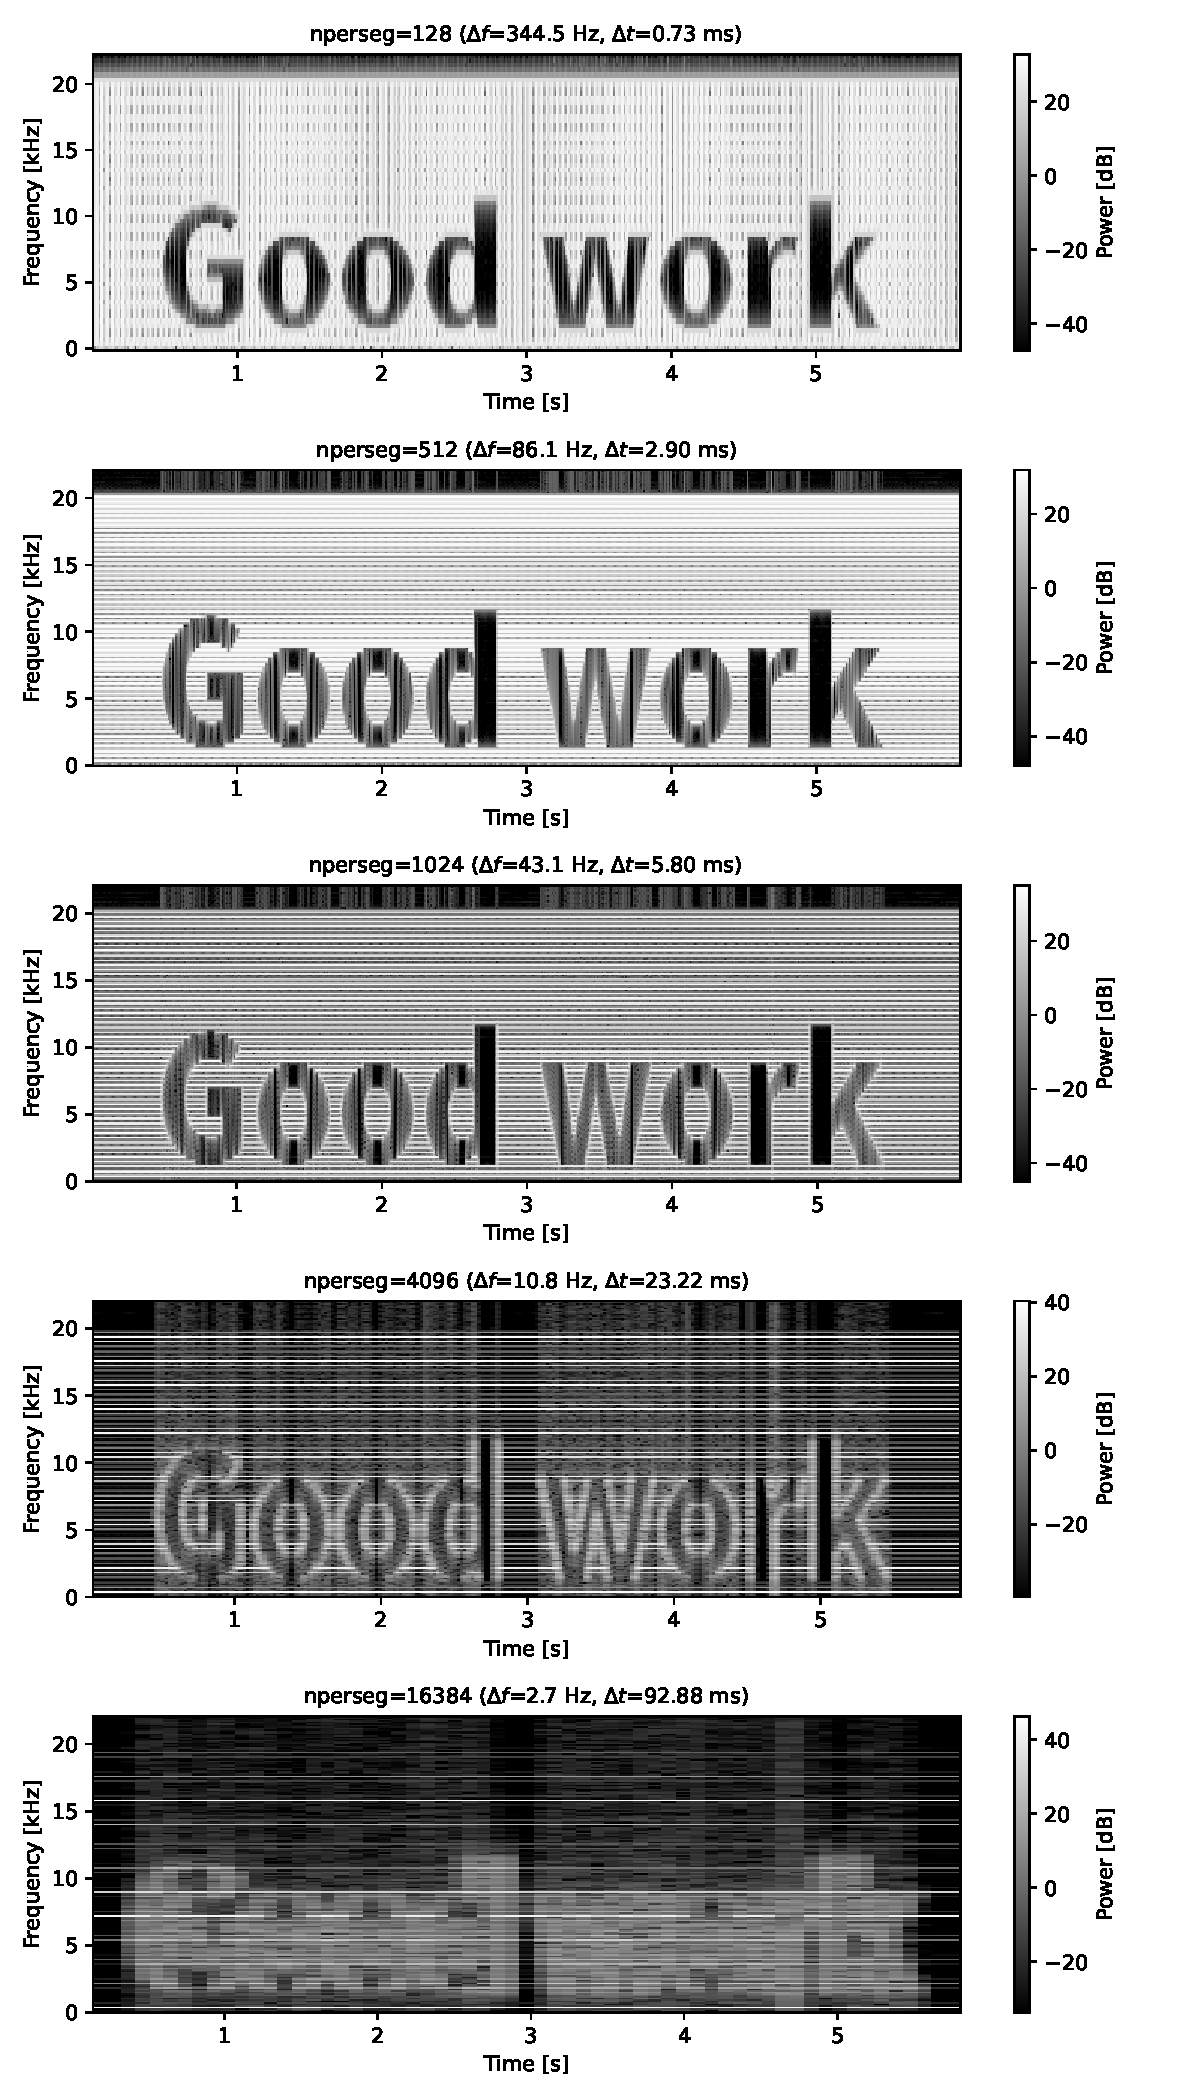
\includegraphics[width=0.72\linewidth]{../experiments/figures/exp02_nperseg_grid.pdf}
\caption{窓長 {\tt nperseg} を変えたスペクトログラムの比較
(ハン窓、オーバーラップ 75\%、dB 表示)}
\label{fig:b2-nperseg}
\end{figure}

\begin{figure}[htbp]
\centering
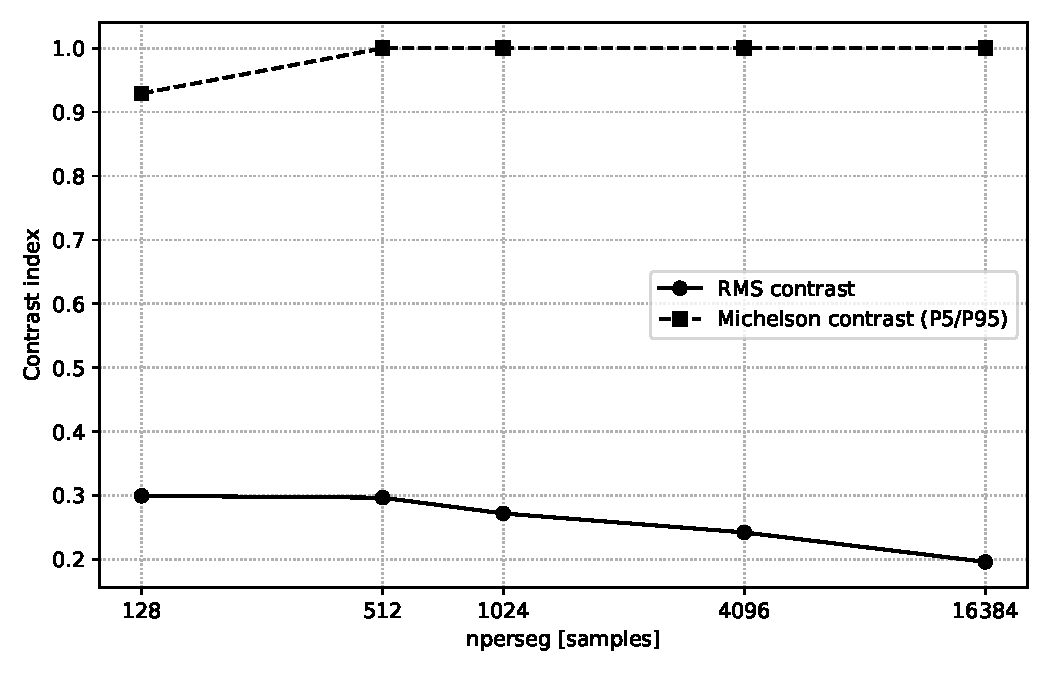
\includegraphics[width=0.75\linewidth]{../experiments/figures/exp02_contrast_vs_nperseg.pdf}
\caption{窓長に対するコントラスト指標の推移(実線: $C_{\mathrm{RMS}}$、
破線: $C_{\mathrm{M}}$)}
\label{fig:b2-contrast}
\end{figure}

この挙動は時間分解能と周波数分解能のトレードオフで説明できる。窓長 $N$ の
窓の時間幅は $T = N/f_s$、周波数ビン間隔は $\Delta f = f_s/N$ であり、
積は $T \cdot \Delta f = 1$ で一定である。すなわち一方を細かくすれば必ず
他方が粗くなる。これは連続時間信号の不確定性関係
$\sigma_t \sigma_f \geq 1/(4\pi)$(ガボール限界)の離散版に相当し、
式 \ref{eq:stft} の窓長 $N$ をどう選んでも両分解能を同時には改善できない。
実測値でも、表 \ref{tab:b2-contrast} の $\Delta f \cdot \Delta t$ は
全窓長で $0.25$(例: {\tt nperseg} $=128$ では
$344.53\ \mathrm{Hz} \times 0.000726\ \mathrm{s} = 0.250$)と
一定であり、格子の細かさの積が保存されていることが確認できる。

判読性が窓長に対して非対称に振る舞う点が本実験の重要な知見である。
図 \ref{fig:b2-nperseg} の文字の縦ストロークの時間幅は約 0.1 秒であるのに対し、
{\tt nperseg} $= 16384$ の窓時間幅は $T = 16384/44100 = 371.5$ ms と
ストローク幅の 3 倍を超えるため、ノッチが窓内で背景雑音と平均化されて
塗りつぶされる。{\tt nperseg} $= 4096$($T = 92.9$ ms)がストローク幅と
同程度となる劣化の始まりであり、実際に $C_{\mathrm{RMS}}$ は基準設定
1024 の 0.2719 から 0.2422 へ低下している。一方、周波数方向は文字の高さが
約 11 kHz、輪郭の構造が 1 kHz 程度と大きいため、{\tt nperseg} $= 128$
($\Delta f = 344.5$ Hz、帯域内ビン数 32)でも判読性は保たれ、
$C_{\mathrm{RMS}}$ は最大の 0.2995 となった。すなわち本音声のメッセージは
周波数分解能よりも時間分解能への要求が厳しく、窓長は小さめに外す方が安全である。
ただし 128 と 512 の差は約 1\%(0.2995 対 0.2966)と小さく、
図の目視では 512--1024 の文字の輪郭が最も鮮明であることから、
$C_{\mathrm{RMS}}$ の微差のみで 128 を最良と断定することはできない。

$C_{\mathrm{M}}$ は 512 以上で 1.0000 に飽和した。これは文字ノッチの画素が
表示下限 $P_{\max} - 80$ dB に到達し、式 \ref{eq:b2-norm} の下限クリップに
よって $I_5 = 0$ となるためであり、
ノッチ深さが表示ダイナミックレンジを超えていることを意味する。
128 でのみ 0.9292 に低下したのは、$\Delta f = 344.5$ Hz の周波数方向の
平滑化によりノッチの一部が表示下限まで下がりきらないためである。

\subsubsection{窓関数の影響とスペクトルリーク}

窓関数を変えた 3 設定の比較を図 \ref{fig:b2-window} に示す。
$C_{\mathrm{RMS}}$ は blackman 0.3063 $>$ hann 0.2719 $>$ boxcar 0.1617 の順と
なり、boxcar(矩形窓)は hann に対して約 41\% 低い。図 \ref{fig:b2-window} でも
boxcar の文字は黒ではなく灰色に浮いており、判読性が明確に劣る。

\begin{figure}[htbp]
\centering
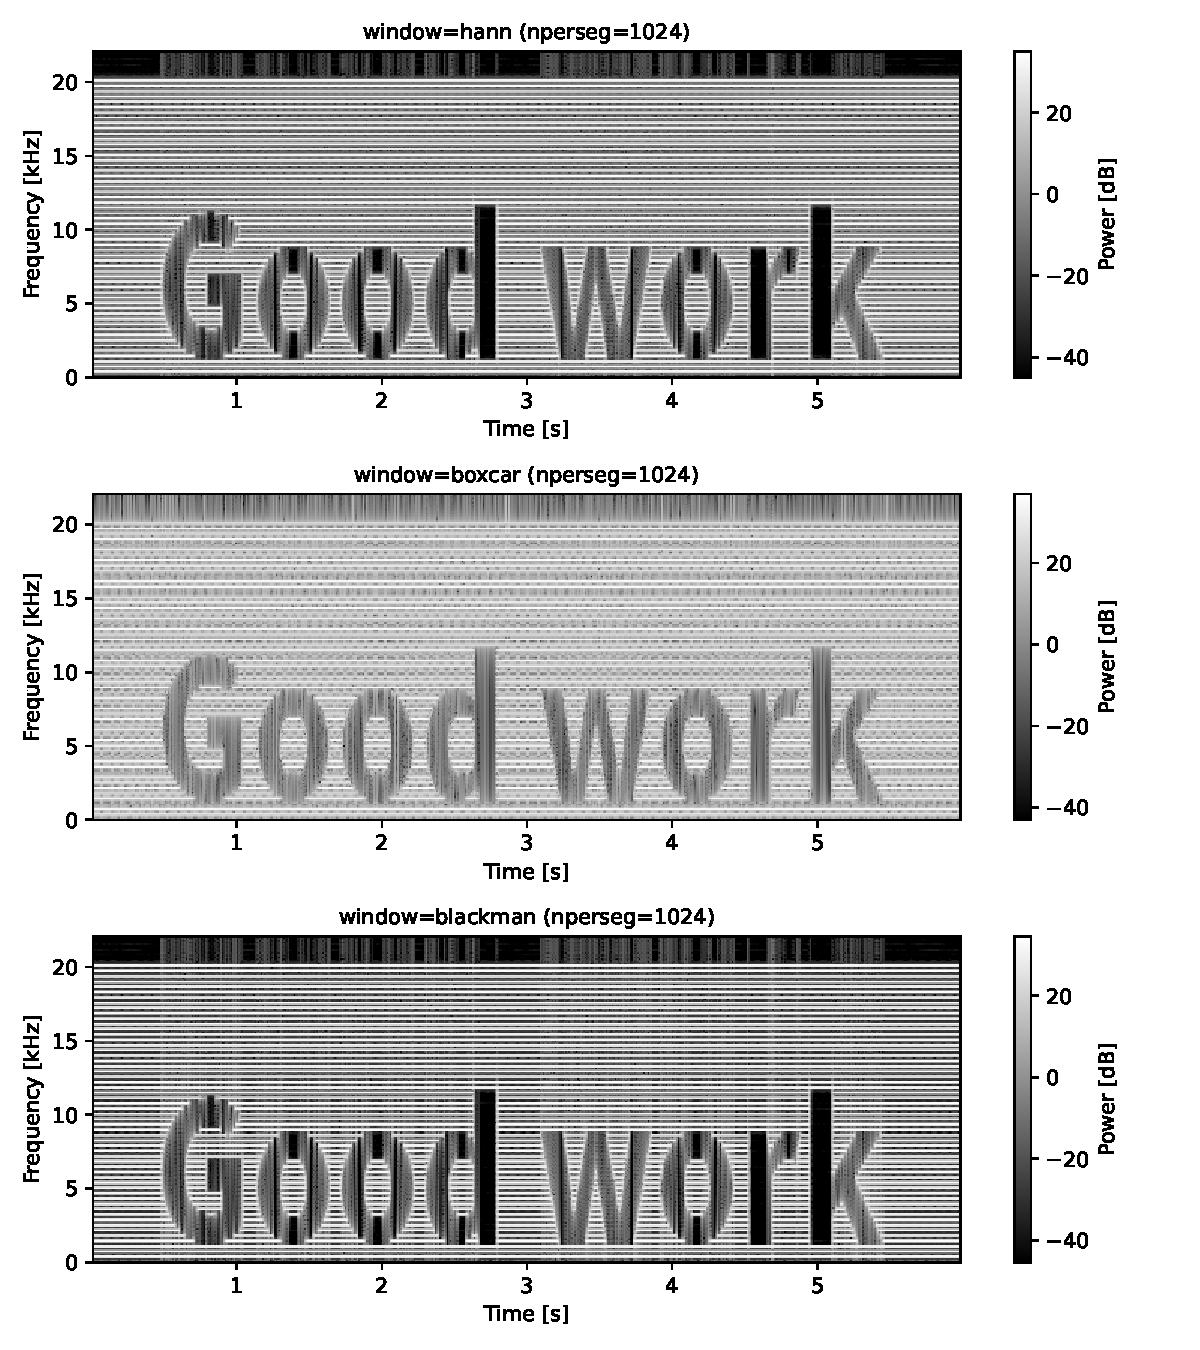
\includegraphics[width=0.8\linewidth]{../experiments/figures/exp02_window.pdf}
\caption{窓関数によるスペクトログラムの比較({\tt nperseg} $=1024$、dB 表示)}
\label{fig:b2-window}
\end{figure}

この差はスペクトルリーク(サイドローブ特性)で説明できる。矩形窓の
第 1 サイドローブは約 $-13$ dB と高く、周囲の帯域の背景雑音のエネルギーが
文字ノッチの周波数ビンへ漏れ込み、ノッチを埋めてしまう。$C_{\mathrm{M}}$ が
boxcar でのみ 0.4101 と大きく低下している($I_5$ が表示下限から浮いている)
ことは、ノッチの底がリークで持ち上げられたことを直接示す。一方 blackman の
サイドローブは約 $-58$ dB と hann(約 $-31$ dB)よりさらに低く、
$C_{\mathrm{RMS}}$ は hann 比で約 12.7\% 向上した。blackman は主ローブ幅が
hann より広く周波数方向のぼけは増えるが、前項で述べたとおり本メッセージは
周波数分解能への要求が緩いため、悪影響が現れない。エネルギーの欠落として
埋め込まれたパターンの可視化では、主ローブ幅よりもサイドローブの低さが
支配的であるといえる。

\subsubsection{表示スケールの影響と指標の性質}

dB 表示と線形表示の比較を図 \ref{fig:b2-scale} に示す。$C_{\mathrm{RMS}}$ は
dB 表示 0.2719 に対し線形表示 0.2230 と約 18\% の低下であった。
5.2.2 項では線形表示によりメッセージ部分とのコントラストが失われると述べたが、
定量実験の結果、本音声に限っては低下は限定的であり判読も可能であった。
これは、メッセージがノッチ型(文字部分のパワーがほぼ 0)で埋め込まれており、
かつ帯域内の背景雑音のパワーが比較的一様であるため、線形スケールでも
文字と背景の差が保たれるからである。成分間のダイナミックレンジが数十 dB に
及ぶ一般の音声・音楽信号では、線形表示は最大成分以外の濃淡を潰すため、
dB 変換の必要性は本実験の結果より大きくなると考えられる。

\begin{figure}[htbp]
\centering
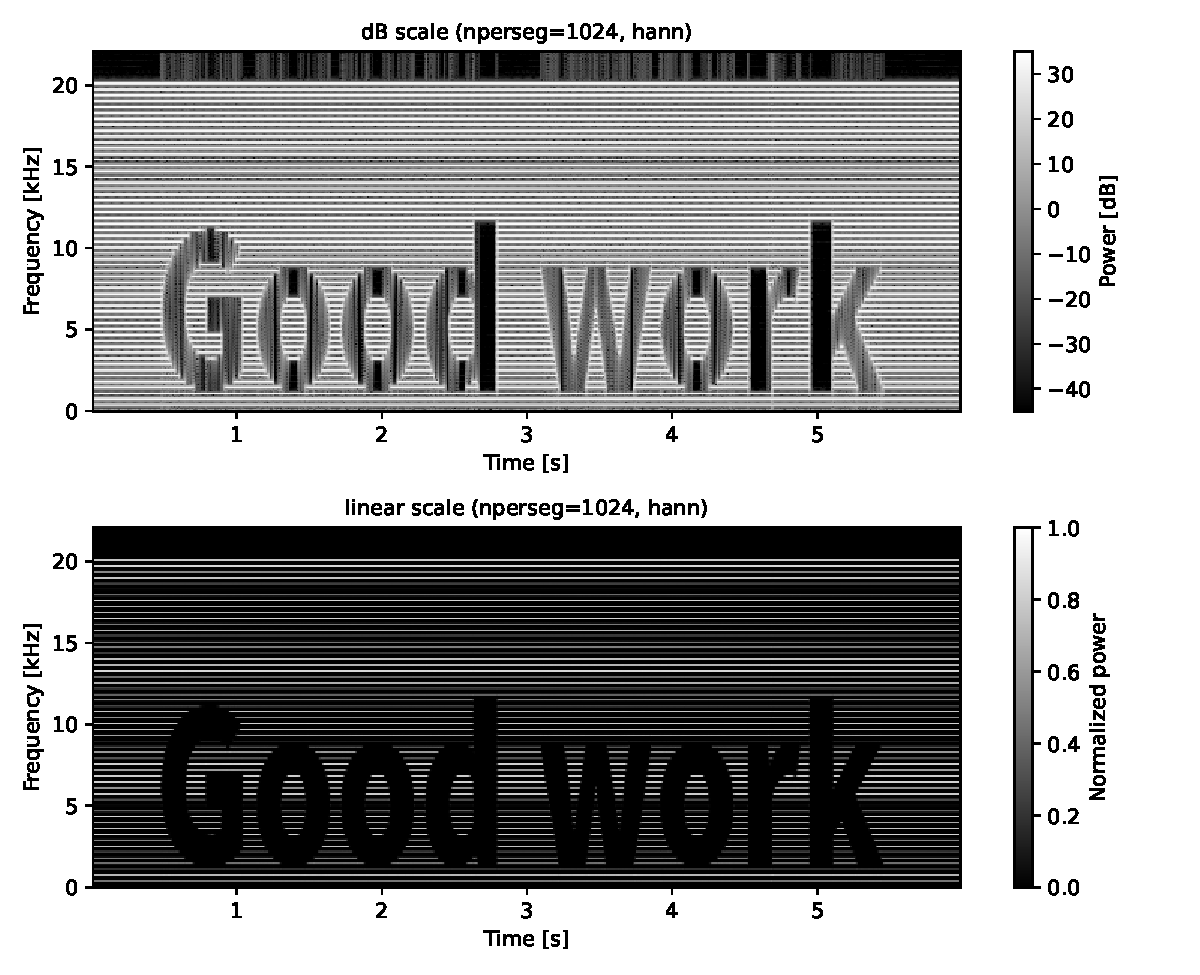
\includegraphics[width=0.85\linewidth]{../experiments/figures/exp02_scale.pdf}
\caption{dB 表示(上)と線形表示(下)の比較({\tt nperseg} $=1024$、ハン窓)}
\label{fig:b2-scale}
\end{figure}

指標の性質にも注意が必要である。表 \ref{tab:b2-contrast} のとおり
$C_{\mathrm{M}}$ は線形表示でも 1.0000 となり、表示の暗さ・濃淡レンジの圧縮を
まったく検出できていない。式 \ref{eq:b2-mic} は分子と分母が画素値に対して
同時にスケールするため、画素値全体が定数倍されても値が変わらない
(スケール不変性)。可読性は紙面上の濃淡差の絶対量に依存するため、
表示画素値の分散を直接測る $C_{\mathrm{RMS}}$(式 \ref{eq:b2-rms})の方が
本目的の指標として適切である。$C_{\mathrm{M}}$ はノッチ深さの飽和判定
(前々項)やリークによる底上げの検出(前項)には有効であり、
2 指標は相補的に用いるべきである。

\subsubsection{最良設定と採用設定の妥当性}

以上を総合すると、測定した範囲での最良設定は blackman 窓・
{\tt nperseg} $= 512$--$1024$・dB 表示($C_{\mathrm{RMS}} = 0.297$--$0.306$)
である。課題 5 で採用したハン窓・{\tt nperseg} $= 1024$・オーバーラップ 75\%・
dB 表示は $C_{\mathrm{RMS}} = 0.2719$ でこれに近く、boxcar($0.1617$)や
{\tt nperseg} $= 16384$($0.1961$)のような判読困難な領域から十分離れた
妥当な設定であったことが定量的に裏付けられた。

また、本音声のようにスペクトログラム上へ視覚パターンを描く埋め込みは、
音声ステガノグラフィの系統的レビュー\cite{b2-steg}における変換領域
(周波数領域)埋め込みの一種と位置づけられる。本実験の結果は、この種の
埋め込みを受信側で復元するための条件を、窓の時間幅 $T$ が
パターンの時間方向の最小構造(本音声では約 0.1 秒)を下回り、かつ
窓関数のサイドローブがノッチ深さに対して十分低いこと、として
数値的に与えるものである。
